\section{Implementation Details}

This section is split to three parts:

\begin{itemize}
\item The first explains the prototype I wrote.
\item The second details implementation challenges when realizing the designed extension and using external libraries.
\item The third shows changes in the extension visible from a user's point of view, with screenshots.
\end{itemize}

\subsection{The prototype}

As mentioned already, the Sharepoint protocol has a brief reference
documentation on MSDN, but that is not enough to create an open-source
implementation of the protocol. To solve that issue, I used two virtual
machines: one running Microsoft Sharepoint 2007, the other running Microsoft
Office 2007, and I used Wireshark\cite{wireshark} to monitor the network
traffic between the two virtual machines.

Trying to reimplement the protocol directly in the LibreOffice extension would
make development slow, partly because that would mean solving UNO interfacing
issues and Java design decisions at the same time, partly because I needed a
simple script to demonstrate how the protocol works, where Java may not be the
best language to use. As a consequence, I decided to write a commandline
prototype in Python, a popular scripting language, and once that was ready and
worked, I ported the logic of the prototype to Java.

The prototype had the following commands:

\begin{itemize}
\item open
\item save
\item save-as
\item delete
\item quit
\item list-versions
\item open-older
\item restore-version
\item delete-version
\item create-space
\item delete-space
\end{itemize}

This covered the functionality outlined in the \emph{Background} section,
except that folder / document listing is implicit here: the open and save-as
operation invoked that, but it had no explicit command assigned.

The prototype also had two switches:

\begin{itemize}
\item The \emph{--alfresco} switch loaded configuration defaults to connect to the Sharepoint emulation interface of Alfresco.
\item The \emph{--test} switch -- which is possible to use at the same with the first one -- executed simple testcases for the above operations.
\end{itemize}

The later switch was critical, so that when I fixed something to work with
Alfresco, I could quickly test I did not break anything in Sharepoint.

Once the used protocol -- at least the parts required by my use-cases -- was
clear, I could begin writing the LibreOffice extension.

\subsection{External libraries}

It was obvious that doing HTTP communication with NTLM authentication is an
already solved problem, but I needed to decide which library to use. Given that
OPAL already used Apache \emph{commons-httpclient}\cite{httpclient} 3.x for
HTTP communication. Unfortunately that version does not support NTLM, so I used
Apache \emph{httpcomponents}\cite{httpcomponents}, which is the successor of
the previous library (starting with version 4.x). The two version series have
different APIs, so it's possible to use both in parallel, and migrating code
incrementally.

Once I had \emph{httpcomponents}, I still needed to write detection code that
decided what to request from \emph{httpcomponents}: Basic or NTLM
authentication.

An other interesting issue was to parse the response received after sending
Vermeer RPC requests to the server. The result is valid HTML, but not XHTML.
For example, part of the response is:

\begin{lstlisting}
<html><head><title>vermeer RPC packet</title></head>
<body>
...
<li>vti_timecreated
<li>TR|27 Feb 2011 19:07:25 +0000
<li>vti_timelastmodified
<li>TR|11 Mar 2011 16:39:35 +0000
<li>vti_timelastwritten
<li>TR|11 Mar 2011 16:39:35 +0000
...
</body>
</html>\end{lstlisting}

That means a simple XML parser was not enough to extract the needed values from
this response. To solve this issue, I used TagSoup\cite{tagsoup}, which is a
SAX parser, accepting plain old HTML input.

\subsection{User Interface}

Once the Sharpeoint Library was ready, I updated the user interface to use the
Sharepoint library for communication. I also had to extend the dialogs to allow
a few more features. Namely:

\begin{itemize}
\item Create and delete document workspaces.
\item Delete documents.
\item Delete and restore versions.
\item When saving a document, allow: minor change with a comment and overwrite of a previous version.
\end{itemize}

For example, creating a new document workspace is implemented as can be seen
here:

\begin{figure}[H]
\centering
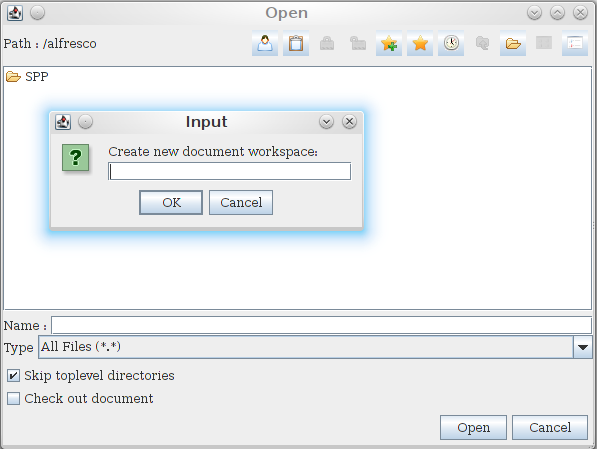
\includegraphics[width=275px,keepaspectratio]{implementation-createdws.png}
\caption{Implementation of creating a document workspace}
\end{figure}

Foo.
